\section{Lezione 6} \hfill 05/03/2026
\subsection{Boschi ripariali}
Anche chiamati ``boschi galleria'', poichè tendono a chiudere (facendo una galleria) sopra il corso d'acqua.\\
Sono fortemente influenzati dalla presenza dell'acqua corrente (es. fiumi, torrenti) e violente, dove può erodere o depositare.\\
Man mano che ci si allontana dalla riva del fiume, le caratteristiche stazionali cambiano:
\begin{itemize}[nosep]
    \item sulla riva dei fiumi ci sono dei NON suoli, che diventano suoli man mano che l'influenza delle piene si riduce;
    \item sull'area più vicina al fiume, dove c'è la massima influenza dell'acqua, non cresce niente;
    \item allontanandosi, c'è l'area influenzata dalle normali piene stagionali (nei periodi primaverili ed autunnali). In queste zone si sviluppano erbe eterofite (che spariranno con la piena);
    \item l'area leggermente più distante è quella delle piene ricorrenti (ogni 3-5 anni, con un tempo di ritorno inferiore ai 10 anni). Le condizioni sono molto buone, che permettono la crescita di salici. La falda è bassa e sopra è presente un suolo primitivo molto permeabile: le piante presenti riescono ad arrivare in falda;
    \item nella fascia successiva le piene diventano più rare, ospitando così la fascia dei salici arborei;
    \item quando ci sono solo le piene eccezionali (20-30 anni), e le condizioni sono più calme, si presenta la farnia.
\end{itemize}
\subsubsection{Salici - Salix}
Specie pioniere, con una forte capacità pollonifera caulinare. La piena distrugge la chioma, ma le radici e la ceppaia ne permettono il ricaccio: si crea la fascia dei salici arbustivi.\\
La rinnovazione avviene perchè la pianta non riesce ad arrivare a maturità sessuale, causa il passaggio delle piene.\\
Quando le condizioni migliorano ancora, ai salici si aggiungono i pioppi (neri e bianchi).
\begin{figure}[htbp]
     \centering
     % Prima Immagine
     \begin{subfigure}[b]{0.33\textwidth}
         \centering
         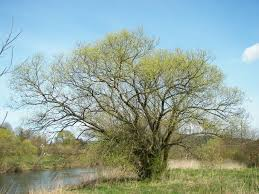
\includegraphics[width=\textwidth]{immagini/salix_alba_portamento.jpg}
        % \caption{}
     \end{subfigure}
     \hfill % Spazio elastico tra le immagini
     % Seconda Immagine
     \begin{subfigure}[b]{0.3\textwidth}
         \centering
         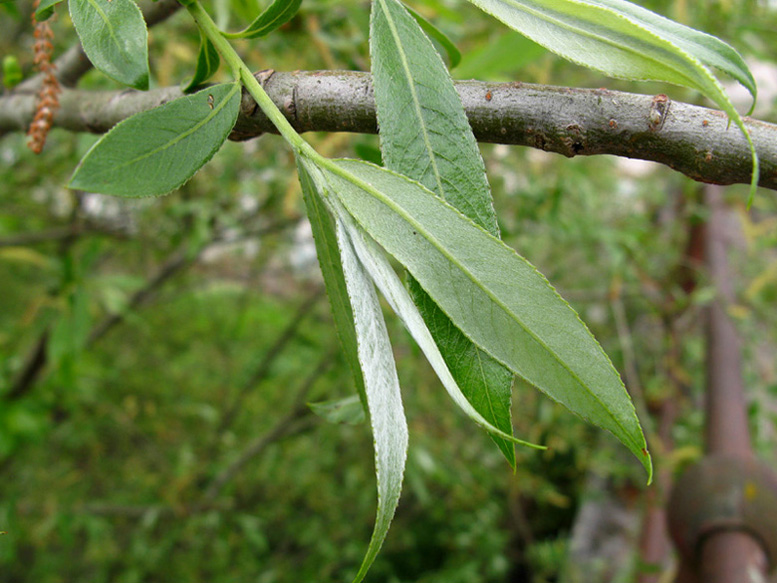
\includegraphics[width=\textwidth]{immagini/salix_alba_foglia.jpg}
         %\caption{}
     \end{subfigure}
     \hfill % Spazio elastico tra le immagini
     % Terza Immagine
     \begin{subfigure}[b]{0.33\textwidth}
         \centering
         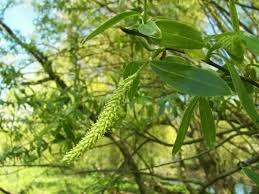
\includegraphics[width=\textwidth]{immagini/salix_alba_fiore.jpg}
         %\caption{}
     \end{subfigure}
     
    \caption{Portamento, foglie e fiore del Salix alba (salice bianco).}
     \label{fig:salice}
\end{figure}
\subsubsection{Pioppo - Populus}
Il pioppo è una specie a rapido accrescimento. È un gran consumatore di acqua, ma non vuole avere l'apparato radicale bagnato; riesce comunque ad approvvigionarsi in falda.\\
Il pioppo nero è più legato alla presenza dell'acqua rispetto al pioppo bianco (quest'ultimo riesce a sopportare l'assenza). La sua foglia è triangolare.\\
Il pioppo bianco ha la corteccia bianca e la pagina inferiore della foglia è lanosa. 
\begin{figure}[htbp]
     \centering
     % Prima Immagine
     \begin{subfigure}[b]{0.33\textwidth}
         \centering
         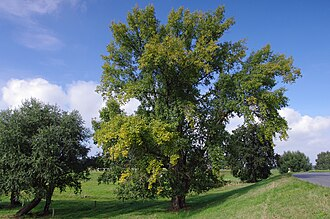
\includegraphics[width=\textwidth]{immagini/popolus_nigra_portamento.jpg}
        \caption{Popolus nigra.}
     \end{subfigure}
     \hfill % Spazio elastico tra le immagini
     % Seconda Immagine
     \begin{subfigure}[b]{0.3\textwidth}
         \centering
         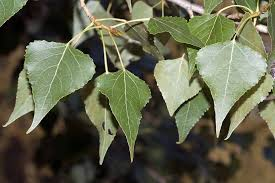
\includegraphics[width=\textwidth]{immagini/popolus_nigra_foglie.jpg}
        \caption{Popolus nigra.}
     \end{subfigure}
     \hfill % Spazio elastico tra le immagini
     % Terza Immagine
     \begin{subfigure}[b]{0.33\textwidth}
         \centering
         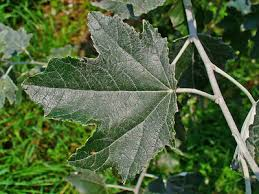
\includegraphics[width=\textwidth]{immagini/popolus_alba_foglie.jpg}
         \caption{Popolus alba.}
     \end{subfigure}
     
    %\caption{}
     \label{fig:popolus}
\end{figure}
\subsubsection{Dalla riva del fiume alla farnia (esclusa)}
Sono formazioni composte da tipiche specie pioniere a vita breve (40-50 anni).\\
Normalmente venivano ceduate ed usate come risorsa energetica legnosa.\\
I fiumi erano, e sono, delle miniere di sabbia. Tendenzialmente c'era un'azione mirata di pulizia dei fiumi: il trasporto fluviale tende a vagare, creando dei meandri. La ceduazione teneva ``pulito'' il bosco: i turni di ceduo di 8-10 anni rendevano ridotti gli assortimenti attorno ai fiumi, rendendo resistenti al passaggio della piena. \\
Con l'arrivo del carbonio fossile, si è smesso di utilizzare i popolamenti attorno ai fiumi; queste formazioni hanno cominciato a crescere ed invecchiare, diventando più suscettibili alle piene.\\
Contemporaneamente, queste formazioni sono importanti aree di rifugio per gli animali e corridori ecologici. \\
La raccolta di questa legna è a macchiatico negativo. Le utilizzazioni devono essere viste come sistemazioni idraulico-forestali, e non come funzione produttiva. 
\subsubsection{Farnia - Quercus robur}
Specie di quercia caducifoglie. Albero di prima grandezza: riesce a raggiungere i 40 metri.\\
Dal punto di vista botanico ha diverse caratteristiche:
\begin{itemize}[nosep]
    \item le branche laterali sono orizzontali e molto grosse;
    \item la corteccia è molto rugosa, e permette di differenziarla dalla rovere (che ha la corteccia più liscia);
    \item le foglie:
    \begin{enumerate}[nosep]
        \item hanno un picciolo cortissimo;
        \item hanno due alette sotto il picciolo;
        \item la larghezza massima è nel terzo superiore;
        \item sono glabre, senza peli;
    \end{enumerate}
        \item le ghiande sono peduncolate (con un lungo picciolo).
\end{itemize}
Ecologicamente ha un comportamento particolare: 
\begin{itemize}[nosep]
    \item ha delle caratteristiche da definitiva:
    \begin{enumerate}[nosep]
        \item seme pesante;
        \item vita lunga, 300-400 anni nell'optimum;
        \item albero di prima grandezza;
    \end{enumerate}
    \item ma anche delle caratteristiche da pioniera:
    \begin{enumerate}[nosep]
        \item fortemente eliofila;
        \item buona capacità pollonifera caulinare.
    \end{enumerate}
\end{itemize}
L'apparato radicale è fascicolato e normalmente profondo. È la migliore pianta forestale per quanto riguarda la resistenza all'acqua dell'apparato radicale.\\
Costituisce dei boschi puri.\\
Il legno che si ottiene: 
\begin{multicols}{2}
\begin{itemize}[nosep]
    \item ha un'ottima combustione;
    \item ha una densità di 0.8;
    \item è di un tipico colore giallastro-bruno;
    \item viene usato per la produzione di infissi, pavimenti, botti;
    \item commercialmente prende il nome di ``rovere'';
    \item permette la produzione di tannini (sia per l'ambito alimentare che per quello farmaceutico).
\end{itemize}
\end{multicols}
Essendo molto eliofila, per rinnovare necessita di molto spazio. In pura teoria, il trattamento selvicolturale da utilizzare sarebbe il taglio raso con il rilascio di riserve. Si dovrebbero fare grandi buche (di almeno 3000 \unit{m^2}, meglio se 0.5 ha); in caso contrario si avrebbe la perdita della farnia.\\\\
Se le condizioni migliorano ancora, i suoli diventano freschi con una giusta dose di acqua, compare il querco-carpineto o il carpineto.
\begin{figure}[htbp]
     \centering
     % Prima Immagine
     \begin{subfigure}[b]{0.25\textwidth}
         \centering
         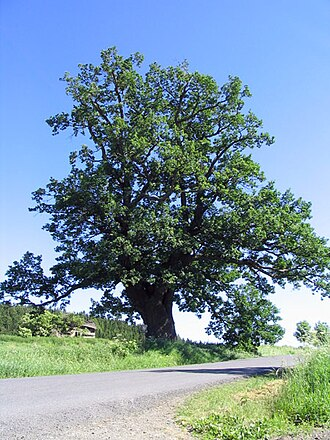
\includegraphics[width=\textwidth]{immagini/quercus_robur_portamento.jpg}
        %\caption{}
     \end{subfigure}
     \hfill % Spazio elastico tra le immagini
     % Seconda Immagine
     \begin{subfigure}[b]{0.3\textwidth}
         \centering
         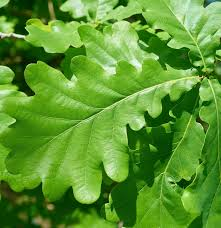
\includegraphics[width=\textwidth]{immagini/quercus_robur_foglie.jpg}
        %\caption{}
     \end{subfigure}
     \hfill % Spazio elastico tra le immagini
     % Terza Immagine
     \begin{subfigure}[b]{0.2\textwidth}
         \centering
         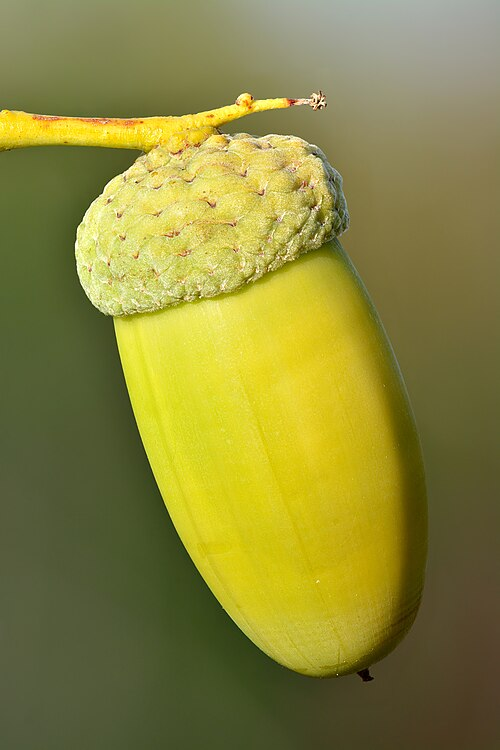
\includegraphics[width=\textwidth]{immagini/quercus_robur_seme.jpg}
         %\caption{}
     \end{subfigure}
     
    \caption{Quercus robur}
     \label{fig:quercus_robur}
\end{figure}
\subsubsection{Querco-carpineto} 
Queste formazioni sono composte principalmente dal carpino bianco (Carpinus betulus) e la farnia (Quercus robur).\\
Queste formazioni, attualmente, hanno principalmente i problemi: 
\begin{itemize}[nosep]
    \item l'estensione areale è molto ridotta, un'ottantina di ha in Veneto (es. Bosco di Carpenedo): aumenta la vulnerabilità in caso di nuove malattie o attacchi parassitari (es. processionaria); 
    \item la farnia ha una areale naturale centro-europeo (es. Svezia, P.P., Nord delle Alpi): gli accrescimenti in P.P. sono maggiori che in Nord-Europa; di conseguenza, il periodo di vita è inferiore. Attualmente, le farnie dell'areale padano hanno sui 60-70 anni, rendendo la generazione di questa specie molto vecchia, e quindi molto vulnerabile.  
\end{itemize}
In passato i querco-carpineti venivano gestiti a ceduo composto: 2 o più specie vengono gestite a ceduo e fustaia (in questo caso il carpino a ceduo e la quercia a fustaia).\\
Il carpino a ceduo aveva turni di 20-30 anni.\\
La fustaia di farnia era disetanea:
\begin{itemize}[nosep]
    \item 60-140 \unit{n/ha};
    \item non c'erano tutte le età (pur essendo disetanea), la quercia si rinnovava quando si ceduava (creando nuovo spazio);
    \item la fustaia aveva classi di 20-40-60-80 anni (se per esempio il ceduo aveva 20 anni).
\end{itemize}
Il carpino è molto competitivo rispetto alla farnia, che da giovane è molto fragile (molto eliofila, vulnerabile ad attacchi funginei, pascolamento).\\
In Francia, data la maggiore area disponibile, i querco-carpineti erano gestiti principalmente a fustaia: i turni erano intorno ai 200 anni (superiore a 140 anni). Venivano svolti tagli successivi: i tagli di sementazione eliminavano tutto il carpino. Le querce rimaste rinnovavano, e successivamente si poteva fare il taglio di sgombero.\\
Oggi c'è il deperimento della farnia, ciò è dovuto ad un sistema di agenti negativi: insetti defogliatori (es. processionaria), competizione con delle altre specie aliene, cambiamento della falda (che in alcuni casi si è alzata o si è abbassata), non è possibile fare la ceduazione normale sennò ci sarebbe l'invasione delle aliene.\\
Oggi sarebbe possibile:
\begin{itemize}[nosep]
    \item aprire grandi buche (difficile, colpa dell'opinione pubblica);
    \item fare delle piantumazioni (necessario comunque aprire per dare spazio alla rinnovazione);
    \item ingrandire le aree (per mitigare i futuri disturbi biotici);
    \item mantenere i popolamenti a solo carpino (avere solamente il carpineto).
\end{itemize}
\subsubsection{Carpino - Carpinus}
Specie definitiva, in P.P. è la specie leader. È sciafila, di seconda grandezza (max 20 m di altezza), la disseminazione è anemocora. La vita è all'incirca di 100-150 anni.\\
L'uso principale è quello legato alla combustione.\\
Il fusto non è perfettamente circolare, corteccia grigia e liscia. La forma del fusto è poco appetita per gli usi di segheria (molto scarto), ed il legno è molto elastico, ma non nervoso. \\
I grandi individui (sopra i 30-40 cm DBH), sono usati per creare i compensati (es. antine della cucina). \\
Solitamente i carpini di grosse dimensioni vengono importati dall'estero.\\
In passato, nel carpineto avveniva una grossa buca, dando così la possibilità alla farnia di entrare e crescere.
\begin{figure}[htbp]
     \centering
     % Prima Immagine
     \begin{subfigure}[b]{0.33\textwidth}
         \centering
         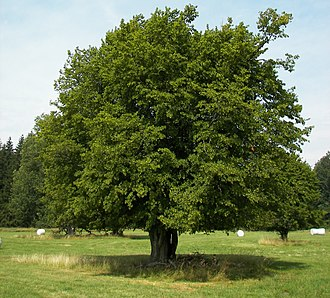
\includegraphics[width=\textwidth]{immagini/carpinus_betulus_portamento.jpg}
        %\caption{}
     \end{subfigure}
     \hfill % Spazio elastico tra le immagini
     % Seconda Immagine
     \begin{subfigure}[b]{0.3\textwidth}
         \centering
         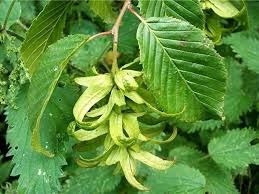
\includegraphics[width=\textwidth]{immagini/carpinus_betulus_foglie.jpg}
        %\caption{}
     \end{subfigure}
     \hfill % Spazio elastico tra le immagini
     % Terza Immagine
     \begin{subfigure}[b]{0.2\textwidth}
         \centering
         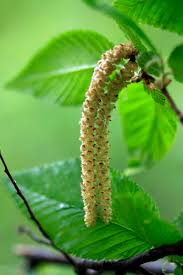
\includegraphics[width=\textwidth]{immagini/carpinus_betulus_peduncolo.jpg}
         %\caption{}
     \end{subfigure}
     
    \caption{Carpinus}
     \label{fig:carpinus}
\end{figure}
\subsubsection{Specie rampicanti}
Sono di due tipi:
\begin{itemize}[nosep]
    \item edera (Hedera helix);
    \item clematide vitalba (Clematis vitalba).
\end{itemize}
Non sono specie parassite, poichè non si nutrono degli alberi sui quali si arrampicano: li usano solamente come supporto per il loro sviluppo (avendo fusti molli e non rigidi).\\
Il ruolo ecologico di queste specie in un sistema forestale è quello di rimuovere le piante deboli.
\paragraph{Edera - Hedera helix}
Normalmente, in un bosco giovane planiziale, striscia per terra; quando necessita di rinnovare (magari per un peggioramento dell'ecosistema attorno), va alla ricerca della luce, arrampicandosi su un supporto. La funzione dell'albero è unicamente quella di supporto fisico.\\
L'edera, essendo sempreverde, è molto appetita per gli erbivori. È mellifera già a gennaio, divenendo una risorsa energetica per le api.\\
Si arrampica sul fusto (fino a 10 m), e non va mai sui rami.\\
Aumenta la massa resistente al vento, portando alla rottura dell'albero.\\
La presenza di edera sul popolamento è un indicatore di condizioni stazionali poco buone.
\paragraph{Clematide vitalba - Clematis vitalba}
Tende a salire sulla chioma e non sul fusto.\\
Una nevicata invernale, assieme alla presenza della Clematide, può portare alla caduta dell'albero.\\\\
Non serve eliminare le specie rampicanti, ma occorre eliminare il problema per il quale le ha portato a salire sugli alberi (solitamente quando la condizione non è ottimale per la luce e per i nutrimenti).
\begin{figure}[htbp]
     \centering
     % Prima Immagine
     \begin{subfigure}[b]{0.33\textwidth}
         \centering
         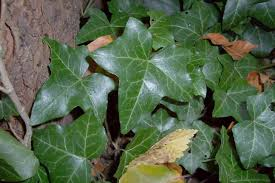
\includegraphics[width=\textwidth]{immagini/hedera_helix_foglie.jpg}
        \caption{Foglie di Hedera helix.}
     \end{subfigure}
     \hfill % Spazio elastico tra le immagini
     % Seconda Immagine
     \begin{subfigure}[b]{0.35\textwidth}
         \centering
         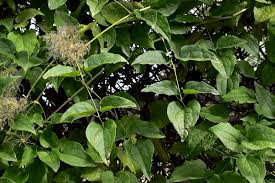
\includegraphics[width=\textwidth]{immagini/clematis_vitalba_foglie.jpg}
        \caption{Foglie di Clematis vitalba.}
     \end{subfigure}
     \hfill % Spazio elastico tra le immagini
     % Terza Immagine
     \begin{subfigure}[b]{0.2\textwidth}
         \centering
         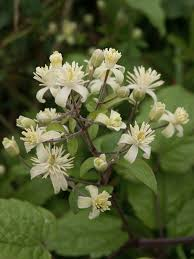
\includegraphics[width=\textwidth]{immagini/clematis_vitalba_fiori.jpg}
         \caption{Fiori di Clematis vitalba.}
     \end{subfigure}
     
    %\caption{}
     \label{fig:clematis_vitalba}
\end{figure}